\documentclass[aspectratio=169,11pt]{beamer}
\usepackage{fontspec}
\setsansfont{texgyreheros}[Extension=.otf,UprightFont=*-regular,BoldFont=*-bold,ItalicFont=*-italic,BoldItalicFont=*-bolditalic]
\usepackage{polyglossia}
\setdefaultlanguage{vietnamese}
\usepackage{tikz,pgfplots,booktabs,array,mathtools}
\usetikzlibrary{arrows.meta,positioning,calc}
\pgfplotsset{compat=1.18,every axis/.append style={font=\scriptsize,axis line style={gray!40},tick style={gray!40},grid=major,grid style={gray!12},legend style={draw=none,fill=none,font=\scriptsize},label style={font=\scriptsize}}}
\definecolor{Navy}{HTML}{14263D}
\definecolor{Red}{HTML}{C82333}
\definecolor{Teal}{HTML}{087E8B}
\definecolor{Amber}{HTML}{C77D19}
\definecolor{Muted}{HTML}{526477}
\setbeamercolor{normal text}{fg=Navy,bg=white}
\setbeamercolor{structure}{fg=Teal}
\setbeamercolor{frametitle}{fg=Navy}
\setbeamercolor{alerted text}{fg=Red}
\setbeamerfont{frametitle}{size=\Large,series=\bfseries}
\setbeamerfont{footline}{size=\tiny}
\setbeamersize{text margin left=9mm,text margin right=9mm}
\setbeamertemplate{navigation symbols}{}
\setbeamertemplate{itemize item}{\color{Teal}\small\textbullet}
\setlength{\parskip}{3pt}
\setbeamertemplate{frametitle}{\vspace{3mm}{\scriptsize\color{Red}\insertsectionhead\par}\vspace{1mm}\insertframetitle\par\vspace{1mm}}
\setbeamertemplate{footline}{\hspace{9mm}\color{Muted}PTIT\enspace /\enspace XỬ LÝ ẢNH SỐ\hfill StarDist\hspace{5mm}\insertframenumber\,/\,27\hspace{9mm}\vspace{3mm}}
\newcommand{\notefoot}[1]{\par\vspace{2mm}{\fontsize{7}{9}\selectfont\color{Muted}#1\par}}
\newcommand{\lead}[1]{\par{\large\bfseries #1}\par\vspace{2mm}}
\newcommand{\pic}[3]{\begin{minipage}[t]{#1\linewidth}\centering\includegraphics[width=\linewidth,height=32mm,keepaspectratio]{assets/#2}\par\vspace{1mm}{\small #3}\end{minipage}}
\newcommand{\stepbox}[2]{\node[draw=Teal!35,fill=Teal!5,rounded corners=2pt,minimum width=28mm,minimum height=12mm,align=center,font=\small] (#1) {#2};}
\newcommand{\OtsuAP}{0.643}
\newcommand{\OtsuAPSD}{0.238}
\newcommand{\OtsuPQ}{0.627}
\newcommand{\OtsuPQSD}{0.208}
\newcommand{\OtsuDice}{0.895}
\newcommand{\OtsuDiceSD}{0.070}
\newcommand{\OtsuMAE}{14.06}
\newcommand{\OtsuMAESD}{25.28}
\newcommand{\OtsuTime}{0.0327}
\newcommand{\OtsuTimeSD}{0.0232}
\newcommand{\WaterAP}{0.715}
\newcommand{\WaterAPSD}{0.199}
\newcommand{\WaterPQ}{0.677}
\newcommand{\WaterPQSD}{0.166}
\newcommand{\WaterDice}{0.894}
\newcommand{\WaterDiceSD}{0.071}
\newcommand{\WaterMAE}{6.94}
\newcommand{\WaterMAESD}{10.56}
\newcommand{\WaterTime}{0.0647}
\newcommand{\WaterTimeSD}{0.0462}
\newcommand{\StarAP}{0.846}
\newcommand{\StarAPSD}{0.132}
\newcommand{\StarPQ}{0.782}
\newcommand{\StarPQSD}{0.117}
\newcommand{\StarDice}{0.915}
\newcommand{\StarDiceSD}{0.050}
\newcommand{\StarMAE}{3.48}
\newcommand{\StarMAESD}{3.79}
\newcommand{\StarTime}{0.3277}
\newcommand{\StarTimeSD}{0.2098}
\newcommand{\BenchmarkRows}{%
Otsu & $0.643\pm0.238$ & $0.627\pm0.208$\\
Watershed & $0.715\pm0.199$ & $0.677\pm0.166$\\
StarDist & $0.846\pm0.132$ & $0.782\pm0.117$\\
}
\newcommand{\ThresholdRows}{%
Otsu & $0.643\pm0.238$ & $0.453\pm0.276$ & $0.223\pm0.221$\\
Watershed & $0.715\pm0.199$ & $0.501\pm0.266$ & $0.214\pm0.207$\\
StarDist & $0.846\pm0.132$ & $0.692\pm0.238$ & $0.305\pm0.313$\\
}
\newcommand{\SecondaryRows}{%
Otsu & 0.895 & 14.06 & $0.0327\pm0.0232$\\
Watershed & 0.894 & 6.94 & $0.0647\pm0.0462$\\
StarDist & 0.915 & 3.48 & $0.3277\pm0.2098$\\
}
\newcommand{\CrossRows}{%
low & 9 / 11 & 0.900 & 0.940\\
median & 157 / 156 & 0.990 & 0.997\\
high & 24 / 24 & 1.000 & 0.998\\
}


\title{Phân đoạn nhân tế bào với StarDist}
\author{Nhóm 03 -- PTIT}
\date{Bài tập lớn Xử lý ảnh kỹ thuật số}
\hypersetup{pdftitle={StarDist | Nhóm 03 | PTIT},pdfauthor={Nguyễn Hồng Quang; Nguyễn Trọng Nam Khánh; Vũ Dũng}}
\begin{document}
\section{BÀI TẬP LỚN / NHÓM 03}
\begin{frame}[plain]
\begin{minipage}{.77\linewidth}{\small\color{Red}\bfseries HỌC VIỆN CÔNG NGHỆ BƯU CHÍNH VIỄN THÔNG}\end{minipage}\hfill
\includegraphics[width=12mm]{assets/ptit-logo.jpg}
\par\vspace{4mm}
{\fontsize{27}{30}\selectfont\bfseries Phân đoạn nhân tế bào\par với \textcolor{Teal}{StarDist}\par}
\par\vspace{3mm}{\large Từ đa giác hình sao đến thực nghiệm Python và Fiji}
\par\vspace{5mm}\par\textcolor{Red}{\rule{20mm}{1.2pt}}\par
{\small Nguyễn Hồng Quang \enspace B23DCVT361\par Nguyễn Trọng Nam Khánh \enspace B23DCCE052\par Vũ Dũng \enspace B23DCVT110}
\vfill{\scriptsize Xử lý ảnh kỹ thuật số \hfill Nhóm 03}
\end{frame}

\section{01 / BÀI TOÁN VÀ THIẾT KẾ THÍ NGHIỆM}
\begin{frame}{Kết quả chính: tách đúng từng nhân}
\begin{columns}[T]
\column{.57\textwidth}
{\fontsize{48}{52}\selectfont\color{Teal}\bfseries\StarAP}\par
AP@0.50 của StarDist trên 50 ảnh test.
\par\vspace{3mm}
\lead{Cao hơn Watershed 0.131 điểm}
Sai số đếm trung bình: \textbf{\StarMAE{} nhân/ảnh}.
\column{.39\textwidth}

\includegraphics[width=\linewidth,height=43mm,keepaspectratio]{assets/crop_stardist_python.png}
\end{columns}\par
\notefoot{Phạm vi: suy luận bằng mô hình pretrained; không huấn luyện lại. Chưa xác minh mức trùng lặp giữa dữ liệu huấn luyện weight và test split. Nguồn: summary\_metrics.csv, $n=50$.}
\end{frame}

\begin{frame}{Từ vùng tiền cảnh đến từng đối tượng}
\pic{.30}{crop_input.png}{Ảnh huỳnh quang}\hfill
\pic{.30}{crop_binary.png}{Semantic: nhân / nền}\hfill
\pic{.30}{crop_gt.png}{Instance: mỗi nhân một ID}
\par\vspace{4mm}
\lead{Hai nhân chạm nhau vẫn phải là hai đối tượng.}
Mục tiêu: phát hiện, phân đoạn và đếm từng nhân; không chỉ tô đúng vùng sáng.
\notefoot{Cùng một vùng cắt 192\,$\times$\,192 pixel của ảnh median. Binary mask được suy ra từ ground truth. Màu thể hiện ID, không phải loại tế bào.}
\end{frame}

\begin{frame}{Dữ liệu và ranh giới đánh giá}
\begin{columns}[T]
\column{.31\textwidth}{\Huge\color{Teal}\bfseries447}\par ảnh trong train split
\column{.31\textwidth}{\Huge\color{Teal}\bfseries30}\par ảnh validation lấy từ train
\column{.31\textwidth}{\Huge\color{Teal}\bfseries50}\par ảnh test để báo cáo cuối
\end{columns}\par
\par\vspace{5mm}
\begin{itemize}
\item 497 cặp ảnh--mask TIFF; lưu SHA-256 để kiểm tra dữ liệu.
\item Validation cố định, seed 42; không giao với 50 ảnh test.
\item Chọn tham số Watershed trên validation; giữ ngưỡng mặc định của model khi benchmark StarDist.
\end{itemize}
\notefoot{DSB2018 trong archive của dự án. Weight 2D\_versatile\_fluo có nguồn huấn luyện từ DSB2018; chưa có danh sách ID huấn luyện weight để chứng minh test độc lập.}
\end{frame}

\begin{frame}{Một giao thức, ba phương pháp}
\centering
\begin{tikzpicture}[>=Latex,node distance=8mm]
\stepbox{input}{Ảnh + GT}
\node[right=9mm of input,align=center,font=\small] (methods) {Otsu\\Watershed\\StarDist};
\node[right=12mm of methods,draw=Teal!35,fill=Teal!5,minimum height=15mm,align=center,font=\small] (labels) {Nhãn instance\\ID nguyên};
\node[right=10mm of labels,draw=Teal!35,fill=Teal!5,minimum height=15mm,align=center,font=\small] (eval) {Một bộ ghép cặp\\và tính chỉ số};
\draw[->,thick,Teal] (input)--(methods);\draw[->,thick,Teal](methods)--(labels);\draw[->,thick,Teal](labels)--(eval);
\end{tikzpicture}\par
\par\vspace{6mm}
\begin{itemize}
\item Mỗi phương pháp giữ tiền xử lý phù hợp, được ghi trong cấu hình.
\item Đánh giá cùng GT và các ngưỡng IoU: 0.50, 0.75, 0.90.
\item Thời gian: tiền xử lý + suy luận + hậu xử lý sau warmup; bỏ I/O.
\end{itemize}
\notefoot{Thiếu ảnh, mask hoặc prediction phải được báo lỗi. Runtime Python đo trên cùng CPU; không xếp hạng với thời gian khởi động lạnh Fiji.}
\end{frame}

\section{02 / NGUYÊN LÝ STARDIST}
\begin{frame}{Dự đoán hình dạng thay vì chỉ dự đoán pixel}
\pic{.30}{crop_input.png}{1. Ảnh đầu vào}\hfill
\pic{.30}{crop_probability.png}{2. Xác suất đối tượng}\hfill
\pic{.30}{crop_stardist_python.png}{3. Các instance sau NMS}
\par\vspace{4mm}
Mỗi vị trí dự đoán một xác suất $p$ và $R$ khoảng cách xuyên tâm. Các đa giác ứng viên được lọc bằng ngưỡng xác suất và NMS.
\notefoot{Bản đồ ở giữa là đầu ra CNN thực của 2D\_versatile\_fluo, không phải ảnh minh họa tổng hợp. Ảnh hiển thị được phóng về cùng vùng nhìn.}
\end{frame}

\begin{frame}{Biểu diễn một nhân bằng đa giác hình sao}
\begin{columns}[c]
\column{.48\textwidth}\centering
\begin{tikzpicture}[scale=1.1,>=Latex]
\coordinate (O) at (0,0);
\draw[fill=Teal!12,draw=Teal,thick] (0:1.8)--(45:1.45)--(90:1.7)--(135:1.3)--(180:1.65)--(225:1.55)--(270:1.25)--(315:1.6)--cycle;
\foreach \a/\r in {0/1.8,45/1.45,90/1.7,135/1.3,180/1.65,225/1.55,270/1.25,315/1.6}{\draw[Red!65,->] (O)--(\a:\r);}
\fill[Navy](O)circle(2pt);\node[below right] at(O){$\mathbf{x}$};\node[above]at(25:1.5){$r_k$};
\end{tikzpicture}\par
\column{.49\textwidth}
\[\theta_k=\frac{2\pi k}{R},\quad k=0,\ldots,R-1\]
\[\mathbf{v}_k=\mathbf{x}+r_k
\begin{pmatrix}\cos\theta_k\\\sin\theta_k\end{pmatrix}\]
\textbf{Điều kiện:} từ tâm đến mọi điểm của vùng đều nằm trong đối tượng.
\par Hợp với nhiều nhân tế bào; khó biểu diễn vùng lõm sâu hoặc hình dạng không star-convex.
\end{columns}\par
\notefoot{Sơ đồ dùng 8 tia cho dễ đọc. Mô hình sử dụng trong thực nghiệm dự đoán 32 tia. Nguồn: Schmidt et al., MICCAI 2018.}
\end{frame}

\begin{frame}{Xác suất mục tiêu và xác suất dự đoán}
\begin{columns}[T]
\column{.48\textwidth}\centering
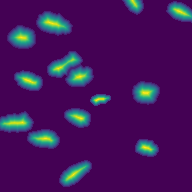
\includegraphics[height=35mm]{assets/crop_edt.png}\par\textbf{Target: EDT chuẩn hóa}\par\small Khoảng cách đến nền, chuẩn hóa riêng trong từng instance; nền bằng 0.
\column{.48\textwidth}\centering

\includegraphics[height=35mm]{assets/crop_probability.png}\par\textbf{Prediction: đầu xác suất CNN}\par\small Giá trị học được; tâm nhân thường có điểm cao hơn vùng sát biên.
\end{columns}\par
\notefoot{EDT là mục tiêu huấn luyện, không phải xác suất dự đoán. EDT tính trên GT đầy đủ rồi mới cắt; hai bản đồ dùng thang viridis từ 0 đến 1.}
\end{frame}

\begin{frame}{Một backbone, hai đầu ra}
\centering
\begin{tikzpicture}[>=Latex,node distance=8mm,font=\small]
\node[draw,minimum height=12mm,align=center](im){Ảnh\\1 kênh};
\node[right=9mm of im,draw=Teal,fill=Teal!7,minimum width=22mm,minimum height=22mm,align=center](enc){Encoder\\giảm mẫu};
\node[right=9mm of enc,draw=Teal,fill=Teal!7,minimum width=22mm,minimum height=22mm,align=center](dec){Decoder\\tăng mẫu};
\node[right=12mm of dec,yshift=9mm,draw=Red,minimum width=30mm,minimum height=10mm](p){$p$: 1 kênh};
\node[right=12mm of dec,yshift=-9mm,draw=Amber,minimum width=30mm,minimum height=10mm](r){$r_k$: 32 kênh};
\draw[->,thick](im)--(enc);\draw[->,thick](enc)--(dec);\draw[->,thick](dec)--(p);\draw[->,thick](dec)--(r);
\draw[->,Teal,thick] (enc.north) to[bend left=35] node[above]{skip connections}(dec.north);
\end{tikzpicture}\par
\par\vspace{4mm}
Đặc trưng nhiều mức kết hợp ngữ cảnh với chi tiết biên. Hai đầu ra cùng mô tả các đa giác ứng viên tại từng vị trí trên lưới.
\notefoot{Sơ đồ nguyên lý U-Net, không biểu diễn toàn bộ lớp và số filter của checkpoint. Model map provenance được lưu trong generated/model\_map\_provenance.json.}
\end{frame}

\begin{frame}{Hàm mất mát: học vị trí và hình dạng}
\[\mathcal{L}=\mathcal{L}_{\mathrm{prob}}+\lambda\mathcal{L}_{\mathrm{dist}}\]
\begin{columns}[T]
\column{.47\textwidth}\lead{Xác suất đối tượng}
\[\mathcal{L}_{\mathrm{prob}}=\operatorname{BCE}(p,\hat p)\]
Target mềm dựa trên EDT giúp ưu tiên vị trí bên trong đối tượng.
\column{.49\textwidth}\lead{Khoảng cách xuyên tâm}
\[\mathcal{L}_{\mathrm{dist}}\propto\sum_{\mathbf{x},k}p(\mathbf{x})\,|r_k-\hat r_k|\]
Sai số tuyệt đối có trọng số foreground; mô hình học hình dạng từ các tia.
\end{columns}\par
\notefoot{Công thức mô tả hai thành phần chính; không khai triển hạng regularization ở nền. Bài tập sử dụng checkpoint pretrained, không báo cáo một quá trình huấn luyện mới. Nguồn: Schmidt et al., 2018.}
\end{frame}

\begin{frame}{NMS và IoU đánh giá là hai phép đo khác nhau}
\begin{columns}[c]
\column{.40\textwidth}\centering
\begin{tikzpicture}
\draw[fill=Teal!12,draw=Teal,thick](0,0)rectangle(3,3);
\draw[fill=Red!30,draw=Red,thick](1,1)rectangle(2,2);
\node[Teal] at(2.5,2.5){$A$};\node[Red]at(1.5,1.5){$B$};
\end{tikzpicture}\par
\column{.57\textwidth}
\textbf{NMS StarDist2D:}
\[o(A,B)=\frac{|A\cap B|}{\min(|A|,|B|)}=1\]
\textbf{Ghép prediction với GT:}
\[\operatorname{IoU}(A,B)=\frac{|A\cap B|}{|A\cup B|}=\frac19\]
Giữ ứng viên điểm cao, loại ứng viên chồng lấn vượt ngưỡng NMS.
\end{columns}\par
\notefoot{Ví dụ hình vuông chứa nhau, diện tích 9 và 1. Không thay mẫu số của NMS bằng hợp diện tích. Model: prob\_thresh = 0.479071; nms\_thresh = 0.30.}
\end{frame}

\begin{frame}{Chuẩn hóa cùng percentile, chưa đủ để đồng nhất}
\[x'=\frac{x-P_1(x)}{P_{99.8}(x)-P_1(x)+\varepsilon}\]
\begin{columns}[T]
\column{.47\textwidth}\lead{Python / CSBDeep}
Percentile nội suy tuyến tính của NumPy.\par Mặc định \texttt{clip=False}: giữ cả giá trị ngoài $[0,1]$.
\column{.49\textwidth}\lead{Fiji / Java CSBDeep 0.6}
Percentile từ histogram.\par Chặn dưới tại 0; không chặn trên tại 1 trong cấu hình đã tái lập.
\end{columns}\par
\par\vspace{3mm}\textcolor{Red}{\textbf{Hệ quả:}} cùng weight và ngưỡng vẫn có thể cho nhãn khác nhau.
\notefoot{Cấu hình benchmark lưu normalization metadata. Không suy diễn rằng Python và Java có đầu vào số học hoàn toàn giống nhau.}
\end{frame}

\section{03 / BASELINE VÀ CÁCH ĐO}
\begin{frame}{Baseline: từ ngưỡng sáng đến tách vùng chạm}
\begin{columns}[T]
\column{.48\textwidth}\centering
\includegraphics[height=33mm]{assets/crop_otsu.png}\par\textbf{Otsu + thành phần liên thông}\par\small Ngưỡng toàn cục; nhân chạm nhau dễ bị gộp.
\column{.48\textwidth}\centering
\includegraphics[height=33mm]{assets/crop_watershed.png}\par\textbf{Watershed có marker}\par\small Dùng cực đại distance transform để tách; nhạy với vị trí và số marker.
\end{columns}\par
\notefoot{Cùng crop của ảnh median. Màu prediction khớp GT khi ghép được tại IoU $\geq0.5$; prediction không khớp tô coral. Tham số min\_distance của Watershed được chọn là 9 trên validation.}
\end{frame}

\begin{frame}{Ghép một--một để phát hiện lỗi tách và gộp}
\begin{columns}[c]
\column{.43\textwidth}\centering
\begin{tikzpicture}[font=\small]
\draw[fill=Teal!15,draw=Teal](0,1.5)rectangle(3,2.5);\node at(1.5,2){1 GT};
\draw[fill=Amber!20,draw=Amber](0,0)rectangle(1.5,1);\draw[fill=Red!15,draw=Red](1.5,0)rectangle(3,1);\node at(.75,.5){P1};\node at(2.25,.5){P2};
\draw[->,thick,Teal](.75,1.5)--(.75,1.05);\draw[dashed,Red](2.25,1.5)--(2.25,1.05);
\end{tikzpicture}\par
\column{.53\textwidth}
Hai nửa có IoU $=0.5$ với GT. Tại $\tau=0.5$, chỉ một nửa được ghép:
\[TP=1,\quad FP=1,\quad FN=0\]
\[F_1=\frac23,\qquad AP_\tau=\frac12\]
Mask nhị phân vẫn có Dice $=1$.
\end{columns}\par
\notefoot{Hungarian tối ưu số cặp đạt ngưỡng trước, sau đó tối ưu IoU; không cho phép nhiều prediction cùng nhận một GT. Ví dụ lý tưởng để phân biệt Dice foreground với chất lượng instance.}
\end{frame}

\begin{frame}{Mỗi chỉ số trả lời một câu hỏi}
\small\renewcommand{\arraystretch}{1.65}
\begin{tabular}{@{}>{\raggedright\arraybackslash}p{24mm}>{\raggedright\arraybackslash}p{62mm}>{\raggedright\arraybackslash}p{47mm}@{}}\toprule
Chỉ số & Định nghĩa & Câu hỏi\\\midrule
$AP_\tau$ & $TP/(TP+FP+FN)$ & Tách đúng bao nhiêu instance?\\
$F_1$ & $2TP/(2TP+FP+FN)$ & Phát hiện cân bằng thế nào?\\
$PQ_\tau$ & $\sum_{\mathrm{matched}} IoU/(TP+\frac12FP+\frac12FN)$ & Đúng instance và sát biên?\\
Dice & $2|M_p\cap M_g|/(|M_p|+|M_g|)$ & Foreground trùng bao nhiêu?\\
MAE đếm & $\operatorname{mean}|N_p-N_g|$ & Sai lệch số nhân mỗi ảnh?\\\bottomrule
\end{tabular}\par
\notefoot{$AP_\tau$ dùng theo StarDist matching accuracy tại một ngưỡng IoU, không phải diện tích dưới đường precision--recall của COCO. Các kết quả tổng hợp là mean trên ảnh.}
\end{frame}

\begin{frame}{Chọn Watershed trên validation}
\begin{columns}[c]
\column{.64\textwidth}
\begin{tikzpicture}\begin{axis}[width=\linewidth,height=47mm,xlabel={min\_distance (pixel)},ylabel={Mean AP@0.50},xmin=2,xmax=12,ymin=.45,ymax=.76,xtick={3,5,7,9,11}]
\addplot[Teal,very thick,mark=*] table[x=distance,y=ap]{generated/watershed.dat};
\addplot[only marks,Red,mark=*,mark size=3pt] coordinates{(9,.708947)};
\end{axis}\end{tikzpicture}\par
\column{.32\textwidth}{\Huge\color{Red}\bfseries9}\par min\_distance được chọn\par\par\vspace{3mm}$AP=0.709\pm0.254$\par trên 30 ảnh validation.
\end{columns}\par
\notefoot{Đường biểu diễn mean; số $\pm$ là SD giữa các ảnh. Chỉ chọn trong tập \{3,5,7,9,11\}; không dùng test split để điều chỉnh. Nguồn: dsb2018\_benchmark/watershed\_validation\_sweep.csv.}
\end{frame}

\section{04 / KẾT QUẢ THỰC NGHIỆM}
\begin{frame}{StarDist dẫn đầu về chất lượng instance}
\centering
\begin{tikzpicture}\begin{axis}[width=123mm,height=47mm,ybar,bar width=11pt,ymin=0,ymax=1.07,xtick={0,1,2},xticklabels={Otsu,Watershed,StarDist},ylabel={Mean trên 50 ảnh},legend style={at={(.02,.98)},anchor=north west},enlarge x limits=.25]
\addplot[fill=Teal,draw=Teal,error bars/.cd,y dir=both,y explicit] table[x=x,y=ap,y error=ap_sd]{generated/benchmark.dat};
\addplot[fill=Amber,draw=Amber,error bars/.cd,y dir=both,y explicit] table[x=x,y=pq,y error=pq_sd]{generated/benchmark.dat};
\legend{AP@0.50,PQ@0.50}
\end{axis}\end{tikzpicture}\par
\notefoot{Error bar: SD giữa 50 ảnh, không phải khoảng tin cậy. AP StarDist = \StarAP{} $\pm$ \StarAPSD{}; PQ = \StarPQ{} $\pm$ \StarPQSD{}. Nguồn: summary\_metrics.csv.}
\end{frame}

\begin{frame}{Siết IoU: độ chính xác biên vẫn là thách thức}
\centering\renewcommand{\arraystretch}{1.55}
\begin{tabular}{@{}lccc@{}}\toprule
Phương pháp & AP@0.50 & AP@0.75 & AP@0.90\\\midrule
\ThresholdRows\bottomrule
\end{tabular}\par
\par\vspace{5mm}\par\raggedright
\lead{Phát hiện đúng chưa đồng nghĩa biên trùng khít.}
StarDist giữ thứ hạng đầu, nhưng AP giảm còn 0.305 khi yêu cầu IoU $\geq0.90$.
\notefoot{Mean $\pm$ SD trên cùng 50 ảnh. SD lớn tại ngưỡng cao cho thấy mức độ khác nhau giữa các ảnh; không diễn giải như độ ổn định đã được bảo đảm.}
\end{frame}

\begin{frame}{Độ trùng vùng, sai số đếm và chi phí tính toán}
\centering\small\renewcommand{\arraystretch}{1.55}
\begin{tabular}{@{}lccc@{}}\toprule
Phương pháp & Dice $\uparrow$ & MAE đếm $\downarrow$ & Giây/ảnh $\downarrow$\\\midrule
\SecondaryRows\bottomrule
\end{tabular}\par
\par\vspace{4mm}\raggedright
\lead{Đổi thêm thời gian để giảm lỗi đếm.}
StarDist giảm MAE từ 6.94 xuống 3.48 so với Watershed; chạy chậm hơn trên cấu hình CPU này.
\notefoot{Dice và MAE: mean; thời gian: mean $\pm$ SD. Intel Core i5-8257U 1.40 GHz, macOS 15.7, Python 3.11.9. Warmup trước đo; không gồm đọc/ghi ảnh. Không dùng số liệu này để so tốc độ với Fiji.}
\end{frame}

\begin{frame}{Cùng một ảnh: nhìn rõ khác biệt giữa các phương pháp}
\centering
\pic{.185}{median_input.png}{Đầu vào}\hfill\pic{.185}{median_gt.png}{Ground truth}\hfill\pic{.185}{median_otsu.png}{Otsu}\hfill\pic{.185}{median_watershed.png}{Watershed}\hfill\pic{.185}{median_stardist_python.png}{StarDist}
\par\vspace{5mm}\raggedright
Otsu có xu hướng gộp vùng chạm. Watershed cải thiện việc tách. StarDist dùng hình dạng học được để phân đoạn các nhân dày đặc.
\notefoot{Ảnh median cố định từ bộ ba minh họa lịch sử, không phải ảnh được chọn lại để làm đẹp kết quả. Cùng màu biểu diễn cặp prediction--GT được ghép; coral là prediction không ghép được tại IoU 0.50.}
\end{frame}

\begin{frame}{Fiji: quy trình độc lập, kết quả tái lập được}
\begin{columns}[T]
\column{.55\textwidth}
\lead{Ảnh $\to$ StarDist2D $\to$ Label TIFF}
Model 2D\_versatile\_fluo, percentile 1/99.8 và các ngưỡng được ghi rõ trong macro/config.
\par Tái chạy bằng Java 8 + Maven với native TensorFlow 1.12 đúng nền tảng.
\par\textcolor{Teal}{\textbf{3/3 nhãn tái chạy trùng từng pixel với nhãn Fiji lịch sử.}}
\column{.40\textwidth}\centering
\includegraphics[height=40mm]{assets/crop_fiji.png}\par\small Nhãn Fiji trên crop median
\end{columns}\par
\notefoot{Đây là bằng chứng tái lập Fiji so với Fiji lịch sử, không phải bằng chứng Fiji trùng Python. Kết quả và hash: results/fiji\_rerun/reproduction\_check.csv.}
\end{frame}

\begin{frame}{Fiji--Python: hai ca đạt, một ca cần giải thích}
\begin{columns}[c]
\column{.62\textwidth}\small\renewcommand{\arraystretch}{1.7}
\begin{tabular}{@{}lccc@{}}\toprule
Ca & $N_{Py}/N_{Fiji}$ & $F_1$ & Dice\\\midrule
\CrossRows\bottomrule
\end{tabular}\par
\par\par\vspace{3mm}Tiêu chí: $F_1\geq0.95$ và Dice $\geq0.95$.\par
\textcolor{Red}{\textbf{Ca low không đạt: Fiji thêm 2 instance.}}
\column{.34\textwidth}\centering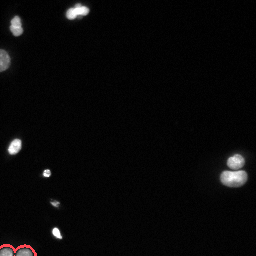
\includegraphics[width=\linewidth,height=41mm,keepaspectratio]{assets/low_unmatched.png}\par\scriptsize Hai vùng không ghép được được khoanh màu.
\end{columns}\par
\notefoot{Ghép trực tiếp hai bộ nhãn tại IoU 0.50; $n=3$, không suy rộng cho toàn bộ 50 ảnh. Khác biệt chuẩn hóa và xử lý biên là các yếu tố cần kiểm soát, chưa kết luận nhân quả. Nguồn: cross\_platform/comparison.csv.}
\end{frame}

\begin{frame}{Độ nhạy tham số trên 30 ảnh validation}
\begin{columns}[T]
\column{.49\textwidth}\centering\small\textbf{Ngưỡng xác suất}\par
\begin{tikzpicture}\begin{axis}[width=\linewidth,height=40mm,xlabel={$p_{\min}$},ylabel={Mean AP@0.50},xmin=.28,xmax=.72,ymin=.76,ymax=.88,xtick={.3,.4,.5,.6,.7}]
\addplot[Teal,thick,mark=*]table[x=value,y=ap]{generated/probability.dat};\end{axis}\end{tikzpicture}\par
\column{.49\textwidth}\centering\small\textbf{Ngưỡng NMS}\par
\begin{tikzpicture}\begin{axis}[width=\linewidth,height=40mm,xlabel={NMS threshold},xmin=.08,xmax=.52,ymin=.76,ymax=.88,xtick={.1,.2,.3,.4,.5}]
\addplot[Amber,thick,mark=*]table[x=value,y=ap]{generated/nms.dat};\end{axis}\end{tikzpicture}\par
\end{columns}\par
\small Tăng $p_{\min}$ từ 0.3 lên 0.7: số nhân dự đoán giảm 35.47 $\to$ 31.50; FN tăng 3.13 $\to$ 6.47 mỗi ảnh.
\notefoot{Cùng thang trục y để so độ nhạy. Quét $p$: giữ NMS=0.3; quét NMS: giữ $p=0.479071$. Các đường là mean; sweep dùng validation, không thay ngưỡng benchmark cuối.}
\end{frame}

\begin{frame}{Kết luận và giới hạn}
\lead{StarDist phù hợp với bài toán tách nhân chạm nhau.}
\begin{itemize}
\item Trên 50 ảnh đang đánh giá: AP@0.50 = \textbf{0.846}, PQ = \textbf{0.782}; sai số đếm thấp nhất trong ba phương pháp.
\item Fiji tái lập được; đối chiếu trực tiếp với Python còn một ca không đạt tiêu chí tương đương.
\item Giới hạn: giả thiết star-convex, lệch miền ảnh, chưa xác minh test độc lập với dữ liệu huấn luyện weight.
\end{itemize}
\par\vspace{3mm}\textcolor{Teal}{\textbf{Bước tiếp theo:}} kiểm thử trên dataset ngoài DSB2018; đồng nhất tiền xử lý và chính sách biên trước khi kết luận tương đương nền tảng.
\notefoot{Đóng góp của bài tập: giải thích nguyên lý, xây dựng baseline, benchmark có kiểm soát và bộ dữ liệu/kết quả có thể kiểm tra lại.}
\end{frame}

\appendix
\section{PHỤ LỤC / TÁI LẬP VÀ TÀI LIỆU}
\begin{frame}[fragile]{A1. Tái lập từ repository}
\small
\begin{verbatim}
python -m pip install -e '.[dev]'
python -m pip install -r requirements-model.txt
python scripts/verify_submission.py
python -m pytest
cd slides/latex
tectonic main.tex
\end{verbatim}
\par\vspace{2mm}Mã lệnh benchmark và Fiji đầy đủ trong \texttt{docs/06\_tai\_lap.md}.\par
39 test đã kiểm tra logic ghép cặp, hình học, tiling và pipeline; coverage kết hợp 88\% ở lần kiểm tra của bản hoàn thiện.
\notefoot{Biên dịch slide không cần chạy lại model: PNG và bảng dữ liệu đã đóng gói trong thư mục LaTeX. Cần XeLaTeX hoặc Tectonic; không dùng pdfLaTeX vì font Unicode tiếng Việt.}
\end{frame}

\begin{frame}{A2. Cấu hình cần giữ cố định}
\small\renewcommand{\arraystretch}{1.45}
\begin{tabular}{@{}p{44mm}p{89mm}@{}}\toprule
Thành phần & Giá trị trong thực nghiệm\\\midrule
Checkpoint & 2D\_versatile\_fluo; 32 tia\\
Ngưỡng model & probability = 0.479071; NMS = 0.30\\
Chuẩn hóa Python & percentile 1 / 99.8; clip=False\\
Đánh giá & IoU = 0.50 / 0.75 / 0.90; ghép một--một\\
Watershed & min\_distance = 9; chọn trên 30 ảnh validation\\
Python model stack & Python 3.11.9; StarDist 0.9.1; TensorFlow 2.15.1\\
Fiji tái lập & Java 8; TensorFlow native 1.12; cấu hình Maven\\\bottomrule
\end{tabular}\par
\notefoot{Hash checkpoint, manifest dữ liệu, cấu hình chạy và môi trường chi tiết được lưu cùng kết quả. Boundary policy được ghi riêng cho từng runtime; không mặc định hai triển khai xử lý biên giống nhau.}
\end{frame}

\begin{frame}{A3. Tài liệu nền tảng và nguồn kiểm chứng}
\small
\textbf{[1]} Schmidt et al. (2018). \emph{Cell Detection with Star-convex Polygons}. MICCAI. DOI: \href{https://doi.org/10.1007/978-3-030-00934-2_30}{10.1007/978-3-030-00934-2\_30}.
\par\textbf{[2]} Ronneberger et al. (2015). \emph{U-Net: Convolutional Networks for Biomedical Image Segmentation}. MICCAI.
\par\textbf{[3]} Otsu (1979). \emph{A Threshold Selection Method from Gray-Level Histograms}. IEEE TSMC.
\par\textbf{[4]} Vincent \& Soille (1991). \emph{Watersheds in Digital Spaces}. IEEE TPAMI.
\par\textbf{[5]} Kirillov et al. (2019). \emph{Panoptic Segmentation}. CVPR.
\par\textbf{[6]} \href{https://github.com/stardist/stardist}{StarDist official repository} \enspace /\enspace \href{https://imagej.net/plugins/stardist}{ImageJ StarDist documentation}.
\notefoot{Tài liệu đầy đủ: references/references.bib. Bảng và biểu đồ trong deck lấy từ CSV của repository; hình dự đoán lấy từ nhãn hoặc output CNN thực, không dùng số liệu minh họa.}
\end{frame}
\end{document}
